\section{The God of the Metaphysicians}

\begin{quotationx}
Even as regards those truths about God which human reason could have discovered, it was necessary that man should be
taught by a divine revelation; because the truth about God such as reason could discover, would only be known by a few,
and that after a long time, and with the admixture of many errors.  \flright{\emph{Summa Theologiae}, I.1.1}

Any “dualism”, whether of the theological order like that attributed to the Manicheans, or of the philosophical order
like that of Descartes, is a radically false conception. \flright{\textsc{Rene Guenon}}

\end{quotationx}

\begin{wrapfigure}{tr}{.35\textwidth}
 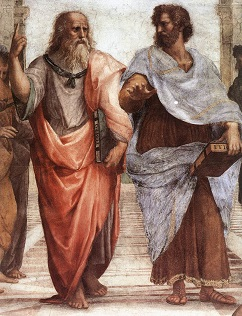
\includegraphics[scale=2.1]{a20151103TheGodofTheMetaphysicians-img001.jpg} 
\end{wrapfigure}

It is said that St Jerome was severely chastised for preferring to read the pagan philosophers rather than Sacred
Scriptures\footnote{\url{http://catholicharboroffaithandmorals.com/St.\%20Jerome.html}}. So it is with some caution that I turn to the pagans, not to commend them, but rather because such writings
have been a great part of my own personal equation. In particular, I am interested in those systems that assume the
intelligibility of the world through thought. These have been known as “Absolute Idealism” or “Monism”. We prefer the
first term, not always used in the strict sense; moreover, they have more of a “family resemblance” and not a totally
common teaching. In short, it represents the Platonic thread in philosophy rather than the Aristotelean. \textbf{Joseph
Marechal}, in \emph{Studies of the Psychology of the Mystics}, compares it to a strict monotheism as the foundation of
a certain type of mysticism.

It is easy to forget that up until a century again, it comprised what was properly called philosophy for educated men.
Other systems of thought, e.g., materialism, naturalism, etc., are not really philosophies since they deny the primacy
of thought. From Plato and Plotinus, it was revived with the German thinkers. The British then adapted their own
version, e.g., with T H Green, Francis Bradley, Bosanquet, etc. A century ago, it was dominated by the Italians
Benedetto Croce and Giovanni Gentile. Julius Evola, who learned German in order to study the German idealists, was also
an Absolute Idealist. Even Rene Guenon, although he disdained profane philosophy, had points in common with such
systems.

The neglect of Absolute Idealism has allowed inferior ideologies to take hold among the educated classes. Often, the
only alternative to such ideologies are crudely expressed dogmas of the exoteric religions, which seem incredible to
most educated folk. Hence, such writings have a threefold purpose for us.

\begin{itemize}
\item Idealism provides an intellectually sophisticated alternative to naturalism, materialism, and modernism. 
\item It is a “halfway house” between atheism and theism. 
\item It provides a safeguard against anthropomorphic and other misconceptions about God. Some idealists identify the
Absolute with God, while others do not. 
\end{itemize}

\paragraph{Surprised by Joy}
C S Lewis was one such person who journeyed from atheism to Absolute Idealism to theism, which he described in
\emph{Surprised by Joy}. \emph{The Magdalen Metaphysicals} describes the intellectual climate at Oxford during
Lewis' time there.

\paragraph{The Vindication}
A recent promoter of Absolute Idealism was \textbf{Timothy Sprigge}. He provides an updated defense of it in the
\emph{Vindication of Absolute Idealism}. In \emph{James and Bradley} and the \emph{God of Metaphysics}, Sprigge
provides a helpful survey of rationalist and idealist philosophies. In the latter book, he outlines how such a
metaphysical system might relate to religion. Unfortunately, I cannot review that chapter here. However, those who have
a religious sensibility, but are turned off by the various alternatives available, may gain something from such an
abstract presentation.

\paragraph{Self-Realization}
Following Bradley, Sprigge claims that self-realization is the goal of life. Of course, that makes sense if we interpret
that in Guenon's notion of the actualization of all of man's possibilities, including the
transcendent possibilities. Ultimately, that is, self-realization is the realization of the Self.

\paragraph{Panpsychism}
Sprigge defends panpsychism, which is the view that the world consists of experiences. For him, there is no dead, or
unexperienced, matter, everything is alive. A more recent example, using a different argument, is \emph{Mind and
Cosmos} by \textbf{Thomas Nagel}, which is reviewed here\footnote{\url{https://www.gornahoor.net/?p=8373}}. Thus, life, consciousness, and thought do not arise from
matter, since the psyche is a fundamental component of the cosmos. Guenon makes a similar claim, since he includes life
as one of the irreducible elements of the world.

\paragraph{Infinite Minds}
In \emph{Infinite Minds: A Philosophical Cosmology}, \textbf{John Leslie} derives a system from Plato's idea
of the Good. \textbf{Hugh Rice}, in \emph{God and Goodness}, develops that idea more fully. He claims that the
Scientific Outlook and Objective Values prove the existence of God. Rather than oppose God to Science, Rice claims that
the scientific outlook requires three beliefs, which transcend the objects of scientific study:

\begin{enumerate}
\item A belief in order 
\item A belief in rationality 
\item A belief in intelligibility 
\end{enumerate}
Then, he demonstrates that there is objective value in the world. From that, he concludes that since it is good for the
world to exist, then it necessarily exists.

Leslie builds on Plato, Spinoza, Bradley, and others, to create an idealist system. Interestingly, he acknowledges the
problem I mentioned at the top: how can you make such metaphysical ideas comprehensible to the modern mind?

\begin{quotex}
Trying to introduce ideas like these in the twenty first century and in the West, one never knows where to start. The
points I want to make could seem entirely natural to a traditionally educated Hindu, or to Hegelians such as Bradley,
or to a physicist such as David Bohm, who speculated that all the parts of our universe form a collective mind of some
sort; yet they can easily be dismissed as preposterous, for all kinds of powerful reasons. … One has to paint a huge
picture at speed, conscious that every brushstroke can earn raised eyebrows, incredulous stares, or worse. One has to
do this because the elements in the picture make sense only when seen as a whole. From which it follows, unfortunately,
that whatever one begins with can look outlandish. 

\end{quotex}

Leslie identifies the things in the world as “the structures of various thoughts in the divine mind”. He goes on to
claim that “when God contemplates various physical possibilities in full detail they do not remain merely possible...
they are genuinely real, existent, actualized, non-fictitious.”

Readers here will recognize these as Guenon's “possibilities of manifestation”, which, in Medieval
metaphysics, are ideas in the Divine Mind. So what goes around, comes around. Unfortunately, the work is marred by an
inadequate understanding of metaphysical Infinity. For this, a reading of Guenon will go a long way to correct.

To get back to the main point, which is that the world exists because it is good for it to exist. This recalls
Bonaventure's journey to God, which surpasses Being to reach the Good. Bonaventure claimed that it is
better for something to exist than not to exist. Here Leslie and Rice seem to be in agreement with Bonaventure.

Nevertheless, for many that proposition may not be so obvious. For example, the Buddha claimed that all life is
suffering and Schopenhauer asserted that it would be better not to exist. In our own time, abortion and euthanasia are
promoted on the grounds that it would be better for some lives not to exist. This topic deserves extended treatment,
but in the meantime, meditate on the Wheel of Fortune Arcanum in the Tarot.

\paragraph{The Idealist View of Life}
That is the title of a book by the Indian philosopher \textbf{Sarvepalli Radhakrishnan}. Radhakrishnan reframes Indian
thought in the terms of Western systems of Absolute Idealism. He does that more thoroughly in the two volumes of
\emph{Indian Philosophy}, quoting Bradley, Gentile, inter alia. In the previous century, European scholars tried to
grasp Hindu philosophy in Western terms. Radhakrishan turns the tables, evaluating Western philosophy in how well it
corresponds to Indian thought. His student, \textbf{T R V Murti}, did the same for Buddhism in \emph{The Central
Philosophy of Buddhism}.

Guenon recommended the study of Eastern thought as the preliminary stage in the recovery of Tradition in the West.
Thinkers like Radhakrishnan, Murti, Aurobindo Ghose, and others, may be a good place to start.

\paragraph{Takeaway}
Obviously, there are many important topics that had to be excluded in this short survey. Some, including
Marechal's work on mysticism\footnote{\url{https://www.gornahoor.net/?p=8467}} and Nagel's on the philosophy of science\footnote{\url{https://www.gornahoor.net/?p=5088}}, will appear in upcoming
posts. However, there is plenty of material to get started on an understanding of the Absolute, the infinite, cosmic
Order, Intelligibility, and Rationality, the Objective Value of Existence, and the goal of Self-Realization.

\flright{\itshape Posted on 2015-11-03 by Cologero}

\begin{center}* * *\end{center}

\begin{footnotesize}\begin{sffamily}

\texttt{themaelstromscup on 2015-11-04 at 12:47 said: }

I may suggest The Elements of Metaphysics by Paul Deussen, which is available for free on Google Books. Duessen was a
follower of Kant and Schopenhauer, as well as an early Sanskrit scholar and friend of Nietzsche. There's
much to be learned from Schopenhauer if one disregards his pessimism, which wasn't a logical consequence of
his system and is easily disentangled therefrom. The aforementioned book is a veritable catechism of Transcendental
Idealism informed by Greek, Christian, and Indian Tradition.


\hfill

\texttt{Cologero on 2015-11-04 at 17:25 said: }

@Maelstrom,\newline
My intent was to focus on recent philosophers writing in English. Nevertheless, I welcome your suggestion.


\hfill

\texttt{aegishjalmer on 2015-11-04 at 19:48 said: }

This post makes me think of a few other points. 

First of all, on the problems of explaining and justifying Idealism, and even philosophy or religion to people today: I
think of Hilaire Belloc and his book Heresy in which he concludes that modernity is the realm of the half educated,
where the masses have been brought up at the expense of the top, which has been brought down. Guenon puts it similarly
in the Reign of Quantity where he speaks of the dynamic of blocking the supernatural and opening up the subnatural,
while Nietzsche speaks of people not being able to think properly, think things through. 

When you consider the conditions under which people are born, the propaganda, false education and spurious myths, and
centuries of decline in various ways (Evola), in which the struggles of Europe via war (etc) leave nowhere to start,
you can see why Guenon recommended the East as a starting point, rather like the Pauline idea of the Gentiles being
grafted onto the tree of Israel. 

Recently this occurred to me as being an essential part of spiritual growth, and I bought a few kindle books on this
exact thing. They look at what a normal human life should be from the point of view of Tradition. I had the distinct
intuition that a large part of our problem today is that we have half conscious instincts and spiritual needs that feed
on traditional archetypes but are blocked and distorted through ignorance (which amounts to saying the normal human
condition of the fall has become modernity's life and is affirmed and justified by it in a negative
response to God's grace, although perhaps it has to do with how Tradition in the West has developed
historically as well), or need proper forms in order to work at all, rather like Jung and his view of dry river beds
needing new streams to flow through them (see his essay Wotan). The books were:

1. The four aims of life in the Tradition of Ancient India by Alain Danielou

2. The Four Goals of Life: a survival guide for the Kali Yuga by Cynkay Morningsong


\hfill

\texttt{David Ravel on 2015-11-05 at 15:03 said: }

Since I am not very well versed in those thinker, I hope this question is not ill-received. 

I always thought that Idealism, when speaking of Plato, was actually a bad translation: it came from the translation of
ousias into idea, which gave rise to a misconception because in actuality, Plato is a realist (ousia being real), not
an idealist (ousia being in the mind (ideation) of the subject) such as Kant. 

When we speak of idealism here, do we speak of Kant or of Plato ? If we speak of both, how do they relate since Kant is
an inversion of Plato in the subject/object relationship ? 

I am confused a bit by all those distinctions. What are we speaking about here when we speak of absolute idealism ?
Thank you.


\hfill

\texttt{Cologero on 2015-11-05 at 17:54 said: }

@David, as I mentioned: “These have been known as “Absolute Idealism” or “Monism”. We prefer the first term, \emph{not
always used in the strict sense}”

I am not interested in picky philosophical disputes. The point is that reason and thinking have been the foundation of
Western philosophy until recently. By the way, I never mentioned Kant, who was not an “Absolute” idealist. For Plato,
the Absolute was the Good.

When I get to the review of Marechal's book on the mystical states associated with various philosophies, the
purpose may become clearer.


\hfill

\texttt{Cassiodorus on 2015-11-05 at 23:56 said: }

According to Guenon, following Shankara, the fundamental distinction is between Atma and Maya, or the Absolute and the
relative. On this view, the personal God who creates and sustains the universe is on the “maya side” of the
Absolute/relative divide. But, as I understand it, the classical theist does not admit of this “maya in Divinis”
doctrine, insisting that the fundamental distinction is between the Creator and the created. I think Christianity may
be compatible with a qualified nondualism like that of the kind espoused by Ramanuja, but I think the unqualified
nondualist traditions are basically patronizing to theists.


\hfill

\texttt{obscure on 2015-11-06 at 00:53 said:} 

Cassiodorus,

One of the fundamental distinctions in Aquinas and the other schoolmen is between the imperfect infinity of matter and
the perfect infinity of God. This imperfect infinity of matter (`indefiniteness' if you prefer)
consists of its being simply determinable and only possessing determination in complexity, whereas God possesses
determination simply (self-determination, aseitas). Matter is like a subject without any subjectivity except insofar as
it is determined as an object of God. I doubt I needed to even write this much nor shall I add any further explanation
since I assume that any competent reader understands all that follows.


\hfill

\texttt{Cassiodorus on 2015-11-06 at 10:30 said: }

Obscure, I appreciate your input. I also apologize if my comments betoken an “incompetence”- I only desire to
understand. For the record, I came to the Christian position by way of the Perennialist writers. I've often
wondered why Guenon and Schuon neve cited figures such as Ramanuja and Madhva. Are their objections to Advaita without
merit?


\hfill

\texttt{David Ravel on 2015-11-06 at 11:51 said: }

@Cologero

My goal was not to start a philosophical debate, but rather to understand where I should look into. You did not mention
Kant, but others did in other occasion, which lead to my confusion. I'm trying to learn.


\hfill

\texttt{Cologero on 2015-11-06 at 20:13 said: }

I'm not necessarily recommending any of these sites, but they may be of interest for further research.

Vivekananda wrote this short piece on Paul Deussen. Vivekananda was the major influence on Radhakrishnan. Guenon did not
approve of V for some reason. Nevertheless, his book on Jnana Yoga brings up many of the same themes that interested
Guenon.

The Swedish philosopher Janolof Bengtsson creates an interesting blend of absolute idealism, tradition, and
paleoconservative authors like Russel Kirk and Irving Babbit. An example is The Case for Idealism. He writes:

\begin{quotex}
what I mean when I speak about and defend idealism – as I do when I speak in terms of Western philosophy, trying to
remedy the lamentable situation – is also an idealism of this original, metaphysical, spiritual and, as it were,
uncompromising variety. An idealism that is defined by the affirmation of this absolute truth about God-Being.

\end{quotex}
In Idealism as Alternative to Modernity, he writes:

\begin{quotex}
The optimal resources for the formulation of the idealist contribution to an alternative modernity therefore seem to me
to be those of personal idealism or personal \textbf{absolute idealism} in its most advanced forms. And as I always
point out – both because of the way in which I myself became an idealist and for the sake of corroborating my argument
for the universality of these issues – there are from the beginning, despite, or beyond, the obvious difficulties of
translation and interpretation, \emph{striking similarities with the Western debates between absolute and personal
idealists in the Vedanta tradition in the East}. 

\end{quotex}
It may not be widely known that Anthroposophy sees its roots in Plato, Aristotle, and Thomas Aquinas. Its goal is to
unite the Platonic and Aristotelian streams of thought.

Here is an homage to Timothy Sprigge: Timothy Sprigge: The Last Idealist. Read it with caution since Sprigge held
non-traditional ideas. Nevertheless, his main influence — Spinoza, Schopenhauer, and Santayana — were coincidentally important to my own early development.


\hfill

\texttt{David Ravel on 2015-11-07 at 08:40 said: }

@Cologero

Thank you for those suggestions.

You said earlier that you focused on English philosophers. What would you suggest in French regarding idealism ?


\hfill

\texttt{Cologero on 2015-11-07 at 09:36 said: }

Oh là là, M. Ravel, you've hit upon a favorite topic of mine!

There is Émile Boutroux, often quoted by Evola. Not to overlook the more famous Henri Bergson, who was a favorite of
Valentin Tomberg.

In France, that type of philosophy went by the name of “philosophy of spirit” or “spiritualism” (nothing to do with
seances as it might mean in English).

The main figures are Louis Lavelle and Rene Le Senne.

I assume you know of Maurice Blondel? (whose philosophy of action was known to Evola).

Finally, Lucien Laberthonniere. He insisted that ideas “must be lived”, not just thought about. In Christian Realism and
Greek Idealism (Realisme chretien et idealisme grec), he addresses your initial question. He understands “idealism” as
the intellectualistic heritage of Greek thought, including both Plato and Aristotle (although he finds shortcomings in
that tradition). You see that is also how I have been using the term.

I don't know why the way of thinking represented by the philosophies of spirit and action has been so
neglected.


\hfill

\texttt{David Ravel on 2015-11-07 at 13:40 said: }

@Cologero

I must say that I know very little of contemporary philosophy. Younger, I had read Nietzsche and Schopenhauer, and was
content with that. After reading the ‘traditionalists’, I only read medieval philosophy and
Plato/Aristotle. 

I must say that now I've also read Kant, Husserll, Ricoeur and a few others, but I had stopped at Kant
regarding any kind of idealism, which I thought was very shortcoming (not including the works of Evola on the matter). 

I will read those authors you suggested, especially those french since it is my mother tongue. 

Thank you.


\hfill

\texttt{Mark Citadel on 2015-11-08 at 13:10 said: }

I really connect with what you're saying here about the intelligibility of the world, for it was through
such arguments that I actually came to Christianity. How do you think one can reconcile mysticism in Christianity with
the very logical approach to the world common to Catholic apologetics in particular? Can we successfully marry the
intelligible and the mystical?


\hfill

\texttt{Cologero on 2015-11-08 at 16:50 said: }

As Guenon put it, “mystical experience” may be super-rational, but certainly not irrational. A follow up to this post
will be a review of Joseph Marechal's Psychology of the Mystics. He shows how one's worldview
relates to the experience of the world. Specifically, he will contrast Absolute Idealism with Theism.

Then, of course, there is Bonaventure's Journey of the Soul to God, in six stages. An early stage is the
realization of the intelligibility of the world.


\hfill

\texttt{Olavsson on 2015-11-15 at 12:45 said: }

Re: Mysticism:

From certain reflections by Guenon that I read rather recently, it would seem that his attitude to mysticism was
sceptical. He gives the impression of not having regarded mystical experience very highly. (I refer to the first two
chapters of ‘Perspectives on Initiation’. He admitted that it had its place within Tradition
as a whole, and might be a spiritual path suited to the nature and possibilities of a particular type of man, but that
ultimately, it is a `passive' approach to spirituality deprived of the properly initiatic
elements that would constitute a certain method for actively overcoming the mortal human condition through the interior
realization of higher states. But as far as I can see, this need not necessarily imply that all of the
`mysticist' features must definitely be excluded, only that an exclusively mystical approach is
insufficient and has serious limitations in the case of one specifically aiming for gnosis. (Speaking only for myself,
I have great respect for some historical mystics.) The same, of course, is true for the strictly rational and
intellectual approach, whether we think of theology or philosophy. This point has been stressed more than once in
articles on this site. Rather than simply rejecting such approaches, the esoteric path would integrate in order to
surpass. Every faculty and function of the being should, then, be ordered into proper alignment so as to fully serve
the spiritual work that is our one absolute purpose in this life, so that all levels of inner activity initially
infected by a profane condition are progressively `sacralized' and mastered in an elevated
expression.

I shouldn't forget to thank Cologero for the recommendation of these useful philosophers. They are noted
down for future research. 

Re: Murti's `The Central Philosophy of Buddhism’: Seeing that the author is a Hindu
and not one initiated into actual Buddhist schools (unless I'm very mistaken), would you say that his work
offers an understanding of Madhyamika that most contemporary Buddhist-adherents of Madhyamika would see as objective
and traditional? All the nuances of the various interpretations and approaches to Mahayana philosophy and metaphysics
are still unclear to me. It is a diverse tradition.

A quick thought on `panpsychism’: If not integrated into a vertical metaphysical order, such a
concept may easily just get stuck on the level of maya-samsara or the pantheist mentality.

[Cologero quote:] “Nevertheless, for many that proposition may not be so obvious. For example, the Buddha claimed that
all life is suffering and Schopenhauer asserted that it would be better not to exist.” [...]

Depends upon the context in which life is evaluated. For an existing being, which is a manifested positive, if I may put
it that way, the confrontation with nothingness, non-being, the negative hole in being, the unconscious, the
dissolution into lower darkness, has always been cause for much instinctive anguish, perhaps the primordial anguish
itself. From this point of view, it is clearly better to be, rather than lose oneself in what is less real. However,
existence and life itself becomes the object of privation, of negativity, the negation of what is more Real, when
compared to the Absolute, the Unconditioned, the Unborn principle. It is when the emanation from that Origin, the
positive creative downward flow causing the perpetual cyclical movement of the cosmic `samsara’, is opposed in order to move against the stream as an active return to the Origin, that the natural cycle of
conditioned existence becomes the enemy, the problem. That life must necessarily have suffering as an inherent
component is inevitable, independently of whether one subscribes to Buddhist views specifically. Every being that is
limited by external conditions, that is in need of things, and subject to change, will eventually experience suffering
as a consequence of these conditions. That life as such implies suffering seems to be beyond reasonable dispute. The
question is rather whether this fact must lead us to conclude that life is bad or even evil (as some gnostics
believed), instead of being a positive creative reality that due to its inevitable relativity, limited conditions and
multiplicity of possibilities must have as one of its consequences suffering, and yes, even evil. That these
conditioned modes of existence equal suffering is a good motivation for heroic spiritual struggle aimed at
transcendental freedom, but obviously there is more to the cosmic manifestation than that alone. The very possibility
of attaining within life the supreme awakening into illumination and liberation, affirmed by the Buddha, should perhaps
make us realize that life, even if ordinarily trapping us in a circle leading away from this supreme state rather than
towards it, also is what we choose to make of it. Those who desperately resign in front of life and take their own
lives, for example, perhaps in the hope that they will achieve a nothingness that is preferable to the suffering of
existence, would be wiser to welcome their suffering as an invitation to transcend their miserable condition by
entering the ascending path in life, which is one of the possible ways to actively give form to life determined by a
superior principle. Then the blindfold of illusions will fall away, and we will no longer be subject to slavish
reactions following from relying upon ever-changing impressions of relative conditions, but will have elevated the
centre of our existence to the highest Truth without which life is indeed meaningless.


\hfill

\texttt{Cologero on 2015-11-18 at 18:26 said: }

“Mysticism” has a range of meanings, but I would agree with the formulation you made. In the upcoming post on the
psychology of mysticism, the texts I am relying on confirm what you said about it. Of course, Guenon was a jnani, so
“knowledge”, or “realization”, is what counts, not some beautiful or unusual experiences.

The thing about Murti is that he was familiar with Guenon. His conclusion that the Madhyamika may be more suitable as
the universal vehicle for tradition instead of the Vedanta is certainly worth considering. He wrote:

\begin{quotex}
Mahayana absolutism and the Advaita Vedanta are valuable as providing the basis on which a world-culture can be built.
It is only absolutism that can make for the fundamental unity of existence and at the same time allow for differences.
Catholicity of outlook and tolerance of differences are their very soul; both insist on the universality of the Real
and transcendence of the ego-centric standpoint. The Vedanta, however, is traditional in outloook and is bound to the
authority of the Veda, and perhaps it presupposes a specific milieu in which alone it can thrive. The Mahayana is quite
liberal, and it has proved its capacity to accommodate itself to various religious and social structure, to revitalise
and absorb them. 

\end{quotex}
Your paragraph on suffering proves — perhaps inadvertently — the point. In the realm of Thought,
the cosmos seems perfectly ordered and rational. However, for the Will, it is much more problematic as it encounters
obstacles and faces up to its own weaknesses. The Will is individulized.


\hfill

\texttt{Max on 2016-06-29 at 12:29 said: }

I took hold of this line, that in order to see the world as not just random happenings “one has to paint a huge picture
at speed”. This comes down to conceptions. If someone is not able to see that for themselves, it is very difficult to
paint that picture for them. One can help by pointing in the right direction, but having someone explain it by a sort
of step by step process does not really do it in the end, since it has to be seen as a whole. To a large extent this
comes down to ones capacity to dwell on large or multiple things simultaneously. The better one is able to do this the
more sense things will make. I am not sure to what degree this is by nature, but it should at least be possible to
improve upon it by training. For example I read about someone who was intrigued by other people saying they could dream
in colour although he could not. By determination and effort he then managed to reach the same degree of
“visualization-power”. So an improvement in conceptual areas like this is definitely possible, but it does not come by
itself, meaning that someone who is perfectly happy with regarding the world as some random hell will not get out of
that view unless they actually wish to do so. Most people make up their mind about something and then by solidification
becomes impossible to reach no matter how many indications to the contrary. In the actual world of conflicting wills
this then translates into a kind of hell since everyone is determined to concede nothing to anyone else, and holds firm
that they alone are correct.

However if there is no purpose, why is it so important to hold on to ones own opinions in the first place? Could they
not just vote on which opinion is correct and then stick to it? It seems as if they have already tried that approach
but it does not work out very well since they take some kind of pride in always having different opinions, which means
that the natural distribution, in a mechanical fashion, always tends towards the greatest diversity, while at the same
time resulting in the largest possible number of people feeling oppressed by the other half. I always wondered why in
almost every “free election”, the margin for victory is just a few points, rather than say 90-10. This just shows that
what is debated has nothing to do with reality, since if the right answer was immediately obvious to everyone, we would
not need to vote in the first place. What this means is that when people think we need to vote on something, that means
that they do not understand the issue, and if they do not understand it, they should have no say in it, demonstrating
how the very idea of voting is a joke from the beginning. In a responsible society the options should rather be
something like this: either I understand something in which case I would not agree to merely “vote on it”, or I do not
understand it in which case I would not agree to vote on it for fear of messing up.

\end{sffamily}\end{footnotesize}